%%%%%%%%%%%%%%%%%%%%%%%%%%%%%%%%%%%
%This is the LaTeX ARTICLE template for RSC journals
%Copyright The Royal Society of Chemistry 2014
%%%%%%%%%%%%%%%%%%%%%%%%%%%%%%%%%%%

\documentclass[twoside,twocolumn,9pt]{article}
\usepackage{extsizes}
\usepackage[super,sort&compress,comma]{natbib} 
\usepackage[version=3]{mhchem}
\usepackage[left=1.5cm, right=1.5cm, top=1.785cm, bottom=2.0cm]{geometry}
\usepackage{balance}
\usepackage{times,mathptmx}
\usepackage{sectsty}
\usepackage{graphicx} 
\usepackage{lastpage}
\usepackage[format=plain,justification=raggedright,singlelinecheck=false,font={stretch=1.125,small,sf},labelfont=bf,labelsep=space]{caption}
\usepackage{float}
\usepackage{fancyhdr}
\usepackage{fnpos}
\usepackage[english]{babel}
\usepackage{array}
\usepackage{droidsans}
\usepackage{charter}
\usepackage[T1]{fontenc}
\usepackage[usenames,dvipsnames]{xcolor}
\usepackage{setspace}
\usepackage[compact]{titlesec}
%%%Please don't disable any packages in the preamble, as this may cause the template to display incorrectly.%%%

\def\hl#1{\textcolor{magenta}{#1}}  % Highlighting for changes


\usepackage{epstopdf}%This line makes .eps figures into .pdf - please comment out if not required.

\definecolor{cream}{RGB}{222,217,201}

\begin{document}

\pagestyle{fancy}
\thispagestyle{plain}
\fancypagestyle{plain}{

%%%HEADER%%%
\fancyhead[C]{
\includegraphics[width=18.5cm]{head_foot/header_bar}}
\fancyhead[L]{\hspace{0cm}\vspace{1.5cm}
\includegraphics[height=30pt]{head_foot/journal_name}}
\fancyhead[R]{\hspace{0cm}\vspace{1.7cm}
\includegraphics[height=55pt]{head_foot/RSC_LOGO_CMYK}}
\renewcommand{\headrulewidth}{0pt}
}
%%%END OF HEADER%%%

%%%PAGE SETUP - Please do not change any commands within this section%%%
\makeFNbottom
\makeatletter
\renewcommand\LARGE{\@setfontsize\LARGE{15pt}{17}}
\renewcommand\Large{\@setfontsize\Large{12pt}{14}}
\renewcommand\large{\@setfontsize\large{10pt}{12}}
\renewcommand\footnotesize{\@setfontsize\footnotesize{7pt}{10}}
\makeatother

\renewcommand{\thefootnote}{\fnsymbol{footnote}}
\renewcommand\footnoterule{\vspace*{1pt}% 
\color{cream}\hrule width 3.5in height 0.4pt \color{black}\vspace*{5pt}} 
\setcounter{secnumdepth}{5}

\makeatletter 
\renewcommand\@biblabel[1]{#1}            
\renewcommand\@makefntext[1]% 
{\noindent\makebox[0pt][r]{\@thefnmark\,}#1}
\makeatother 
\renewcommand{\figurename}{\small{Fig.}~}
\sectionfont{\sffamily\Large}
\subsectionfont{\normalsize}
\subsubsectionfont{\bf}
\setstretch{1.125} %In particular, please do not alter this line.
\setlength{\skip\footins}{0.8cm}
\setlength{\footnotesep}{0.25cm}
\setlength{\jot}{10pt}
\titlespacing*{\section}{0pt}{4pt}{4pt}
\titlespacing*{\subsection}{0pt}{15pt}{1pt}
%%%END OF PAGE SETUP%%%

%%%FOOTER%%%
\fancyfoot{}
\fancyfoot[LO,RE]{\vspace{-7.1pt}
\includegraphics[height=9pt]{head_foot/LF}}
\fancyfoot[CO]{\vspace{-7.1pt}\hspace{13.2cm}
\includegraphics{head_foot/RF}}
\fancyfoot[CE]{\vspace{-7.2pt}\hspace{-14.2cm}
\includegraphics{head_foot/RF}}
\fancyfoot[RO]{\footnotesize{\sffamily{1--\pageref{LastPage} ~\textbar  \hspace{2pt}\thepage}}}
\fancyfoot[LE]{\footnotesize{\sffamily{\thepage~\textbar\hspace{3.45cm} 1--\pageref{LastPage}}}}
\fancyhead{}
\renewcommand{\headrulewidth}{0pt} 
\renewcommand{\footrulewidth}{0pt}
\setlength{\arrayrulewidth}{1pt}
\setlength{\columnsep}{6.5mm}
\setlength\bibsep{1pt}
%%%END OF FOOTER%%%

%%%FIGURE SETUP - please do not change any commands within this section%%%
\makeatletter 
\newlength{\figrulesep} 
\setlength{\figrulesep}{0.5\textfloatsep} 

\newcommand{\topfigrule}{\vspace*{-1pt}% 
\noindent{\color{cream}\rule[-\figrulesep]{\columnwidth}{1.5pt}} }

\newcommand{\botfigrule}{\vspace*{-2pt}% 
\noindent{\color{cream}\rule[\figrulesep]{\columnwidth}{1.5pt}} }

\newcommand{\dblfigrule}{\vspace*{-1pt}% 
\noindent{\color{cream}\rule[-\figrulesep]{\textwidth}{1.5pt}} }

\makeatother
%%%END OF FIGURE SETUP%%%

%%%TITLE, AUTHORS AND ABSTRACT%%%
\twocolumn[
  \begin{@twocolumnfalse}
\vspace{3cm}
\sffamily
\begin{tabular}{m{4.5cm} p{13.5cm} }


\includegraphics{head_foot/DOI} & \noindent\LARGE{\textbf{Indium atoms snorkeling in superfluid helium:  Switching the atomic solubility by electronic excitation$^\dag$}} \\
\vspace{0.3cm} & \vspace{0.3cm} \\

 & \noindent\large{Ralf  Meyer,\textit{$^{a}$} Bernhard Thaler,\textit{$^{a}$} Pascal Heim,\textit{$^{a}$} Stefan Cesnic,\textit{$^{a}$} Sascha Ranftl,\textit{$^{a}$} Johann V. Pototschnig,$^{\ast}$\textit{$^{a}$}  Wolfgang E. Ernst,\textit{$^{a}$} Markus Koch,\textit{$^{a}$} and Andreas W. Hauser$^{\ast}$\textit{$^{a}$}} \\
 

\includegraphics{head_foot/dates} & \noindent\normalsize{Combining a He-droplet experiment with computational studies,  we show that the solubility of In atoms in superfluid helium can be modified via electronic excitation. In the electronic ground state of atomic indium, the strengths of the He-In and the He-He interactions are comparable to each other, which renders the In atom `heliophilic' and therefore soluble in helium. However, the optical excitation of the atom from 5p to the 6s and its inherent spatial diffusion of the electronic density distribution forces the now `heliophobic' In atom onto the surface of the helium droplet. The extra amount of energy needed for this process causes a significant blueshift of the adsorption line in the measured spectrum, which is explained and reproduced by a theoretical model based on ab initio calculations and helium density functional theory.} \\

\end{tabular}

 \end{@twocolumnfalse} \vspace{0.6cm}
]
%%%END OF TITLE, AUTHORS AND ABSTRACT%%%

%%%FONT SETUP - please do not change any commands within this section
\renewcommand*\rmdefault{bch}\normalfont\upshape
\rmfamily
\section*{}
\vspace{-1cm}

%%%FOOTNOTES%%%
\footnotetext{\textit{$^{a}$~Institute of Experimental Physics, Graz University of Technology, Petersgasse 16, A-8010 Graz, Austria. E-mail: johann.pototschnig@tugraz.at, andreas.w.hauser@gmail.com}}

%\footnotetext{\dag~Electronic Supplementary Information (ESI) available: [details of any supplementary information available should be included here]. See DOI: 10.1039/b000000x/}

%%%END OF FOOTNOTES%%%

%%%MAIN TEXT%%%%

\section{Introduction}
\hl{Lieber Markus, bitte um reichlich Input hier von Deiner Seite! Johann, bitte auch um Links zu Theoriearbeiten, insbesondere die von Martin Ratschek}
The spectroscopy of atoms or molecules in He nanodroplets has a long tradition and allowed ... 
HENDI als Begriff definieren...
However, most of these studies were dedicated to the investigation of either helliophilic or heliophobic dopants, i.e. species preferring to be either inside or on the surface of the helium nanodroplet. 
For this study we decided to pick a borderline-element...


\section{Computational Details}

\subsection{Ab initio calculation of diatomic potentials}
\hl{Lieber Ralf, bitte hier alles checken und gegebenenfalls aktualisieren.}
The potential energy surface of the He-In diatomic molecule, a necessary ingredient for the He-DFT approach discussed below, is calculated for  the $^2\Pi{}_{1/2}$ ground state and the $^2\Sigma{}_{1/2}$ electronically excited state. We use the Def2-QZVPD family of basis sets. \cite{Rappoport2010} For indium, the basis set was combined with the ECP28MDF effective core potential of the Stuttgart/K\"oln group.\cite{Metz2000}  All ab initio calculations are performed with the MOLPRO software package.\cite{MOLPRO}

A combination of multiconfigurational self consistent field calculations (MCSCF\cite{Knowles1985, Werner1985}) and multireference configuration interaction (MRCI\cite{WK88, KW92}) is applied to the diatomic system in order to capture the very weak van der Waals-type binding between He and In. In the MRCI approach, 3 valence electrons are included in the active space. The core orbitals are optimized in the preceding MCSCF treatment, but are kept doubly occupied.
The active space in the MCSCF and the subsequent computations comprises 3 electrons in 8 shells, with an occupation pattern of (9,4,4,1) `occupied' and (5,2,2,1) `closed' shells in the MOLPRO nomenclature and internal ordering (A$_1$,B$_2$,B$_1$,A$_2$) for the C$_{2v}$ point group. Both He-In curves have been corrected for basis superposition errors due to their significance for the extremely weak attractive interaction in both states.\cite{boys70} The correction gives rise to geometry shifts in the range of about XX~\AA{}. It also reduces the dissociation energies by XX and XX~cm$^{-1}$ in both states, respectively.

\begin{figure}[h!]
  	\begin{center}
 		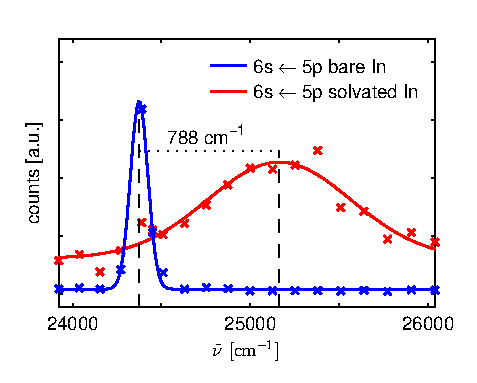
\includegraphics[width=0.45\textwidth]{1.eps}
                \caption{Ab initio PES for the diatomic HeIn molecule in its $^2\Pi{}_{1/2}$ ground and $^2\Sigma{}_{1/2}$ electronically excited state. Both asymptotes have been set to zero energy for a direct comparison of the curvature. The experimental 6s$\leftarrow{}$5p excitation energy for Indium is given by 24 372.957~cm$^{-1}$.\cite{NIST}\label{pic:pes}}
  	\end{center}
\end{figure}

The \emph{ab initio} PES for the HeIn molecule in the $^2\Pi{}_{1/2}$ ground state and the $^2\Sigma{}_{1/2}$ electronically excited state, obtained with the combined CASSCF and MRCI approach described above, are plotted in Figure~\ref{pic:pes}. Both states are very weakly bound with dissociation energies of 3 and 0.5~cm$^{-1}$ for the ground and the excited state, respectively. Note that in both cases the molecular bond is even weaker than the He-He interaction (~7.7 cm$^{-1}$, according to the Aziz potential\cite{Janzen:1997hv} used in the He-DFT ansatz), which already suggests heliophobic behavior on He nanodroplets in both electronic states.  Equilibrium distances of 5.6 and 7.2~\AA{} can be found for the ground and the excited state, respectively. 

\subsection{Helium density functional theory}
The two ab initio PES are then used to calculate the helium density distribution and the free energy of a In-atom-doped He nanodroplet (He$_N$) via helium density functional theory (He-DFT) based on the Orsay-Trento-density functional.\cite{Dalfovo:1995gf} In contrast to DFT approaches of electronic structure theory, this functional is mapping the helium density onto the energy, not the electron density. One-dimensional PES scans of the He$_{N}$-In system can be obtained by a minimization of the free energy as a function of the distance of the In atom from the He$_{N}$ center of mass. The free energy $F[\rho]$ is written as a functional of the helium density $\rho$,
\begin{equation}
  \label{eq:he}
  F[\rho{}] = E[\rho] + U_{\mathrm{ext}}[\rho] - \mu{}N[\rho] - \mathbf{F}\cdot{}\mathbf{R}
[\rho], 
\end{equation}
with $E[\rho]$ denoting the Orsay-Trento-density functional and $U_{\mathrm{ext}}[\rho]$  representing the external interaction potential describing the interaction between the droplet and the indium atom in either the $^2P^{\rm o}_{1/2}$ ground or the $^2S_{1/2}$ electronically excited state. The remaining terms of Equation~\ref{eq:2} reflect two constraints put on the minimization procedure: the conservation of $N$, the particle number, and $\mathbf{R}$, the He droplet mass center.


\begin{figure}[htbp!]
  	\begin{center}
 		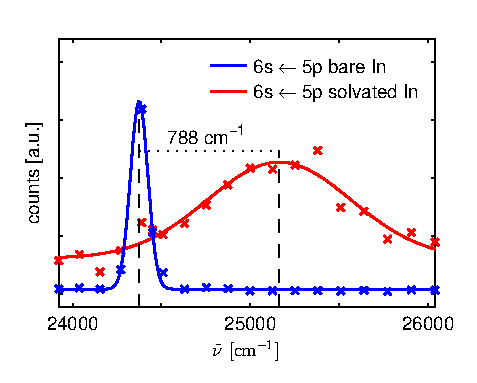
\includegraphics[width=0.45\textwidth]{2.eps}
                \caption{Experimental spectrum for the 6s$\leftarrow{}$5p  transition of In in helium nanodroplets for the bare (blue curve) and the solvated (red curve) atom. A significant blue shift of about 290 cm$^{-1}$ and spectral broadening of the transition line of the atom inside the droplet is observed. \label{pic:exp}}
  	\end{center}
\end{figure}

\section{Experimental Setup}
The experiments were performed on a standard apparatus aiming at spectroscopy of atomic or molecular species inside a superliquid He environment (XXX Zitat?). In short, He$_\mathrm{N}$ were generated via supersonic expansion of high purity (99.9999~\%) helium gas through a pre-cooled nozzle (T$_\mathrm{0}$=17~K, p$_\mathrm{0}$=40~bar, 5 $\mu$m diameter). With these conditions the log-normal distribution of the droplet size predicts a mean number of about 6000 He atoms\cite{Harms1998:dropletsize} per droplet. The beam passes a pickup-chamber, where Indium atoms in vapour phase generated by resistively heated tungsten cells at temperatures around 600$^{o}C$ (vapour pressure <1e-8~mbar) are absorbed. The pickup-conditions are monitored via a quadrupole mass spectrometer (Balzers QMG 422) aligned downstream of the droplet beam and kept optimized for single-atom pickup. After the pickup region the droplets pass a differential pumping stage (DPS), ensuring low base pressures (<1e-9~mbar) in the following main chamber, where ionization with a laser crossed at right angles to the droplet beam takes place. Photoelectrons are collected using a linear time-of-flight (TOF) spectrometer that is also used for the measurement of photoelectrons and/or photoions of molecules in gas phase \cite{Maierhofer:2016acetone}. Electrons are extracted via the combination of a magnetic bottle configuration, ensuring a 4$\pi$ sr collection efficiency, and a small negative (-3~V) repeller voltage. Peaks are decoupled from the anode of a dual-stage microchannel plate detector, amplified and measured with a Stanford Research SR400 counter. Aiming at time resolved experiments, the light-source of choice for photoionization is a commercial Ti:sapphire laser system (Coherent Vitara oscillator and Legend Elite Duo amplifier), which delivers 25~fs pulses of 4~mJ with a central wavelength of 800~nm (fwhm 80~nm) at a repetition rate of 3000~Hz. The pulses are frequency doubled with a 5~mm thick LBO crystal, creating wavelengths around 400~nm with durations in the picosecond time range and a spectral width of 0.8~nm (50~cm$^{-1}$, fwhm). Because Indium has a persistent absorption line around the third harmonic of the Ti:sapphire laser (260~nm)\cite{NIST}, a dispersive prism is used to spatially separate the laser fundamental from the second harmonic in order to avoid this two-photon transition. Absorption spectra around the 6s $\leftarrow$ 5p transition in Indium (24372.956 cm$^{-1}$, 410.18~nm) are taken via tuning the second harmonic wavelength. This is achieved via tilting the crystal axis of the LBO to vary the desired phase matching condition for each wavelength, as was done before in a femtosecond REMPI experiment of molecules in gas phase\cite{koch2017direct}. The laser is focused into the extraction region of the time-of-flight spectrometer with a 1000~mm lens (fused silica), crossing the droplet beam and ionizing the atomic species. In order to avoid non-sequential double ionization, pulse energies are kept low around 2.5~$\mu$J. For each photon energy, electron counts are collected for both the effusive beam (In atoms from the pickup chamber drifting into the interaction region), keeping the valve between the He$_\mathrm{N}$ source chamber and the pickup chamber closed, and for the combined effusive plus droplet beam, keeping the valve open. Signal counts assigned to the solvated In atoms are derived by simply subtracting the measured effusive beam values from the ones where signals from both the bare and the solvated atoms are present. 

\section{Results}
We start with the discussion of our experimental observations. Figure~\ref{pic:exp} shows the experimental spectra along with gaussian fit curves of the 6s$\leftarrow{}$5p electronic excitation of In atoms attached to helium nanodroplets (red curve) and of the bare atomic transition measured with the effusive beam (blue curve). The measured spectral width of the latter (approx. 120~cm$^{-1}$) is significantly bigger than one would expect for an atomic transition, which we explain as a combined influence of the laser bandwidth and saturation effects. The transition line associated with the attached In atoms (red curve, figure \ref{pic:exp}) shows a strong shift to higher energies of approximately 790~cm$^{-1}$ and has a spectral width of about 950~cm$^{-1}$. This significant blueshift and the symmetric broadening of the electronic excitation are characteristics which deviate from the typical spectral features observed for surface-bound dopants such as alkali or alkali earth atoms. \hl{Recherche: Alkalis, AEarth, Al, etc.} This experimental finding suggests a much stronger interaction of the In atom with the helium environment upon electronic excitation, indicating already a full submersion of the atom in its ground state or at least the formation of  more pronounced `dimple' on the droplet surface after pickup.In order to answer this question we develop a theoretical model of the atomic excitation process in the provided He environment. This is done in three steps.

\begin{figure}[htbp!]
  	\begin{center}
 		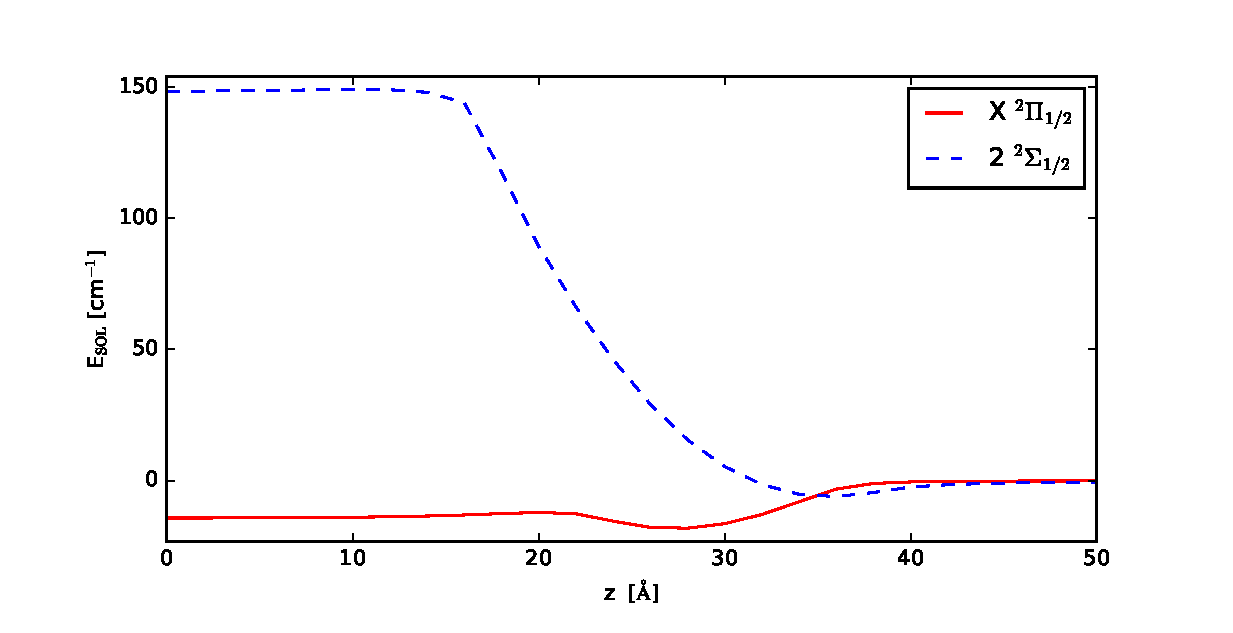
\includegraphics[width=0.45\textwidth]{3.eps}
                \caption{PES scans over the distance between He$_{2000}$ and a single In atom, measured from the helium center of mass. The droplet radius is approximately is approximately 28~\AA. The solid line corresponds to the 5p ground state of the In atom, the dashed line to an 6s excitation.\label{pic:scan}}
  	\end{center}
\end{figure}

First, we fall back on the diatomic He-In potential curves for the two relevant states, and use them to calculate the corresponding external potentials $U_{\rm ext}$ of equation~\ref{eq:he} via a summation over pair potentials. The latter are then used as input for the He-DFT code to obtain helium density distributions as well as total energies for a system consisting of 2000 helium atoms and a single In atom in either the $^2P^{\rm o}_{1/2}$ ground or the $^2S_{1/2}$ electronically excited state. By varying the distance between the In atom and the center of mass of the He nanodroplet, we obtain the one-dimensional PES plotted in Figure~\ref{pic:scan}. As expected from the relatively weak In-He interaction in the $^2S_{1/2}$ electronic state, the In-\ce{He2000} PES shows a clearly heliophobic behavior in the excited state. Defining the solvation energy S(In) of a single In atom in He$_N$ as
\begin{equation}
  \label{eq:solv}
S(\mathrm{In}) = E(\mathrm{In@He}_{N}) - E(\mathrm{He}_{N}),
\end{equation}
we obtain a positive value of XX~cm$^{-1}$ in this case. For indium in its electronic ground state, on the other hand, a negative value of of -XX~cm$^{-1}$ is found, which confirms the heliophilic character in this electronic state. Interestingly, due to qualitatively similar binding energies of He-He and He-In in their electronic ground states, a global minimum near the droplet surface can be observed for indium in its $^2P^{\rm o}_{1/2}$  ground state. This minimum represents a compromise between two counteracting tendencies which underline the uniqueness of the chosen element: On one hand, the system is aiming at maximizing the interaction between the In atom at the He environment. On the other hand, it also tries to keep the perturbations in the He density distribution as small as possible by locking the dopant in an outer region of reduced helium density, effectively avoiding the propagation of density oscillations throughout the whole droplet. Note that the barrier for a full immersion of the In atom is very small (XX cm$^{-1}$). In fact, assuming an initial motion of the In atom at a Landau speed of 56~m/s, i.e. the maximum velocity for frictionless motion in superfluid helium,  we obtain a maximum kinetic energy of approximately XX~cm$^{-1}$, suggesting that those In atoms which remain bound to the droplet after pickup are either located in pronounced dimples near the surface or keep effectively traveling throughout the whole droplet volume. However, even in the latter case, their probability density is also highest near the surface, where the motion of the indium atom has its turning point and the velocity approaches zero.\cite{Hauser:2015cba}

%Also, the solvation energy of -25~cm$^{-1}$ for the In-\ce{He2000} system is not too different from the chemical potential or energy per He atom in a droplet, 7.2~cm$^{-1}$, to which the Orsay-Trento functional has been calibrated\cite{Dalfovo:1995gf} to make this value agree with the measured latent heat of evaporation per particle.\cite{Donnelly1998}

The situation changes completely upon excitation of In from the 5p into the 6s state. Now the In atom perceives a strong radial force towards the droplet surface due to the strongly repulsive character of the excited state PES in Figure~\ref{pic:scan}, which has its origin in extended electron density of the 6s state and proposes the analogy to a lifejacket which makes the In atoms `emerge' from their helium bath. They either leave the droplet or float on its surface for near zero kinetic energies due to a very shallow surface minimum of less than 1.5~cm$^{-1}$.

\begin{figure}[htbp]
  	\begin{center}
 		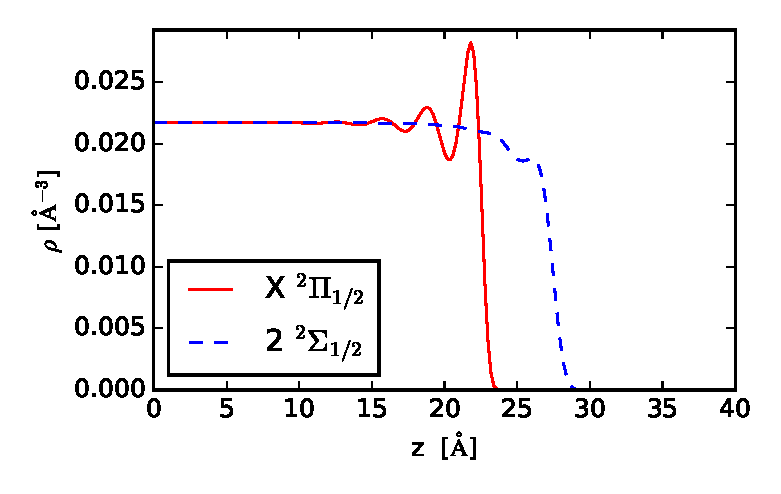
\includegraphics[width=0.45\textwidth]{4.eps}
                \caption{Helium density distribution along the $z$-axis for a pure (dashed) and In-doped (solid) helium nanodroplet consisting of 2000 He atoms, the latter calculated at the minimum free energy internuclear distance for the $^2P^{\rm o}_{1/2}$ ground or the $^2S_{1/2}$ excited state of the indium atom. The helium distribution near the surface is strongly dependent on the electronic state of the In atom. A shorter intermolecular distance and increased He compression are a consequence of the stronger interaction in the electronic ground state.\label{pic:cut}}
  	\end{center}
\end{figure}

Figure~\ref{pic:cut} provides convenient cuts through the helium density of a pure and an In-doped He nanodroplet, showing the density distributions along the intermolecular axis of the In-He$_{2000}$ system (or any radial direction in the case of a pure,  radially symmetric He nanodroplet). The densities for the doped droplet are calculated for the minimum free energy geometries in both studied states of the In-He$_{2000}$ system. Note the compression of the helium due to the interaction with the dopant, which is more pronounced in the electronic ground state of In and appears at shorter intermolecular distance due to the stronger van der Waals interaction between the In atom and its neighboring He atoms. Figure~\ref{pic:cont} shows contour plots of the helium density for both electronic states of the In atom. The formation of a pronounced `dimple' is clearly visible for the $^2P^{\rm o}_{1/2}$ electronic ground state, while the density is barely affected by the In atom in its $^2S_{1/2}$ excited state. 

\begin{figure*}[htbp!]
  	\begin{center}
 		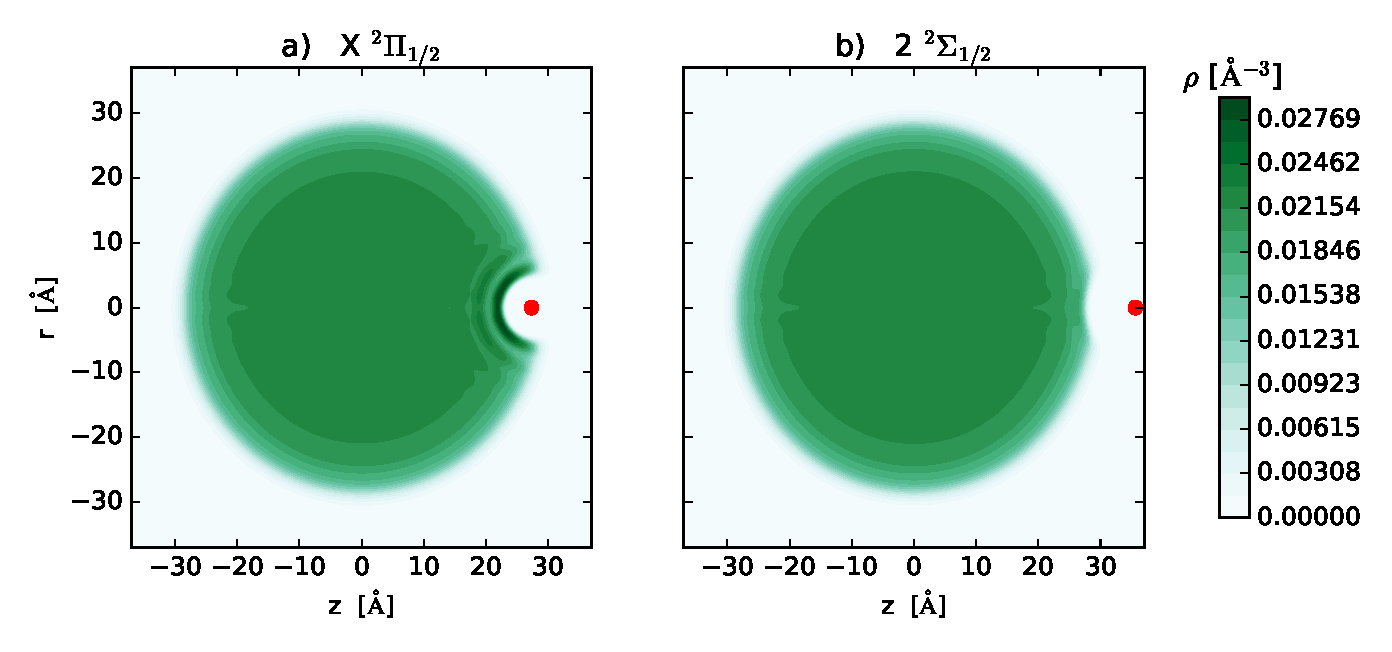
\includegraphics[width=0.95\textwidth]{5.eps}
                \caption{Contour plots of a He$_3000$ nanodroplet with a single In atom in its $^2P^{\rm o}_{1/2}$ ground state (a) and its $^2S_{1/2}$ excited state (b). Note the almost complete immersion of the atom in the electronically excited state.\label{pic:cont}}
  	\end{center}
\end{figure*}

The second step of our modeling approach is dedicated to the electronic excitation of the near-surface immersed In atom. Assuming a vertical excitation, justified by the different timescales for the electronic excitation and the relaxation of the He density, we can estimate the extra energy needed for a 6s$\leftarrow{}$5p transition of a partly immersed In atom by an inversion of the pair-potential technique used to obtain $U_{ \rm ext}$, which is also known as the `frozen-droplet approximation': Assuming no He relaxation at all upon electronic excitation of the In atom, we can calculate this extra energy by a summation of pairwise interactions between He and In in the $^2S_{1/2}$ excited state for the initial helium density distribution $\rho{}_G$ obtain for the electronic ground state of the In atom. Repeating this for various distances between the In atom and the droplet center of mass we obtain this extra energy $\Delta{}E(z)$ needed for electronic excitation as a function of distance as shown in Figure~\ref{pic:extra}.

\begin{figure}[htbp!]
  	\begin{center}
 		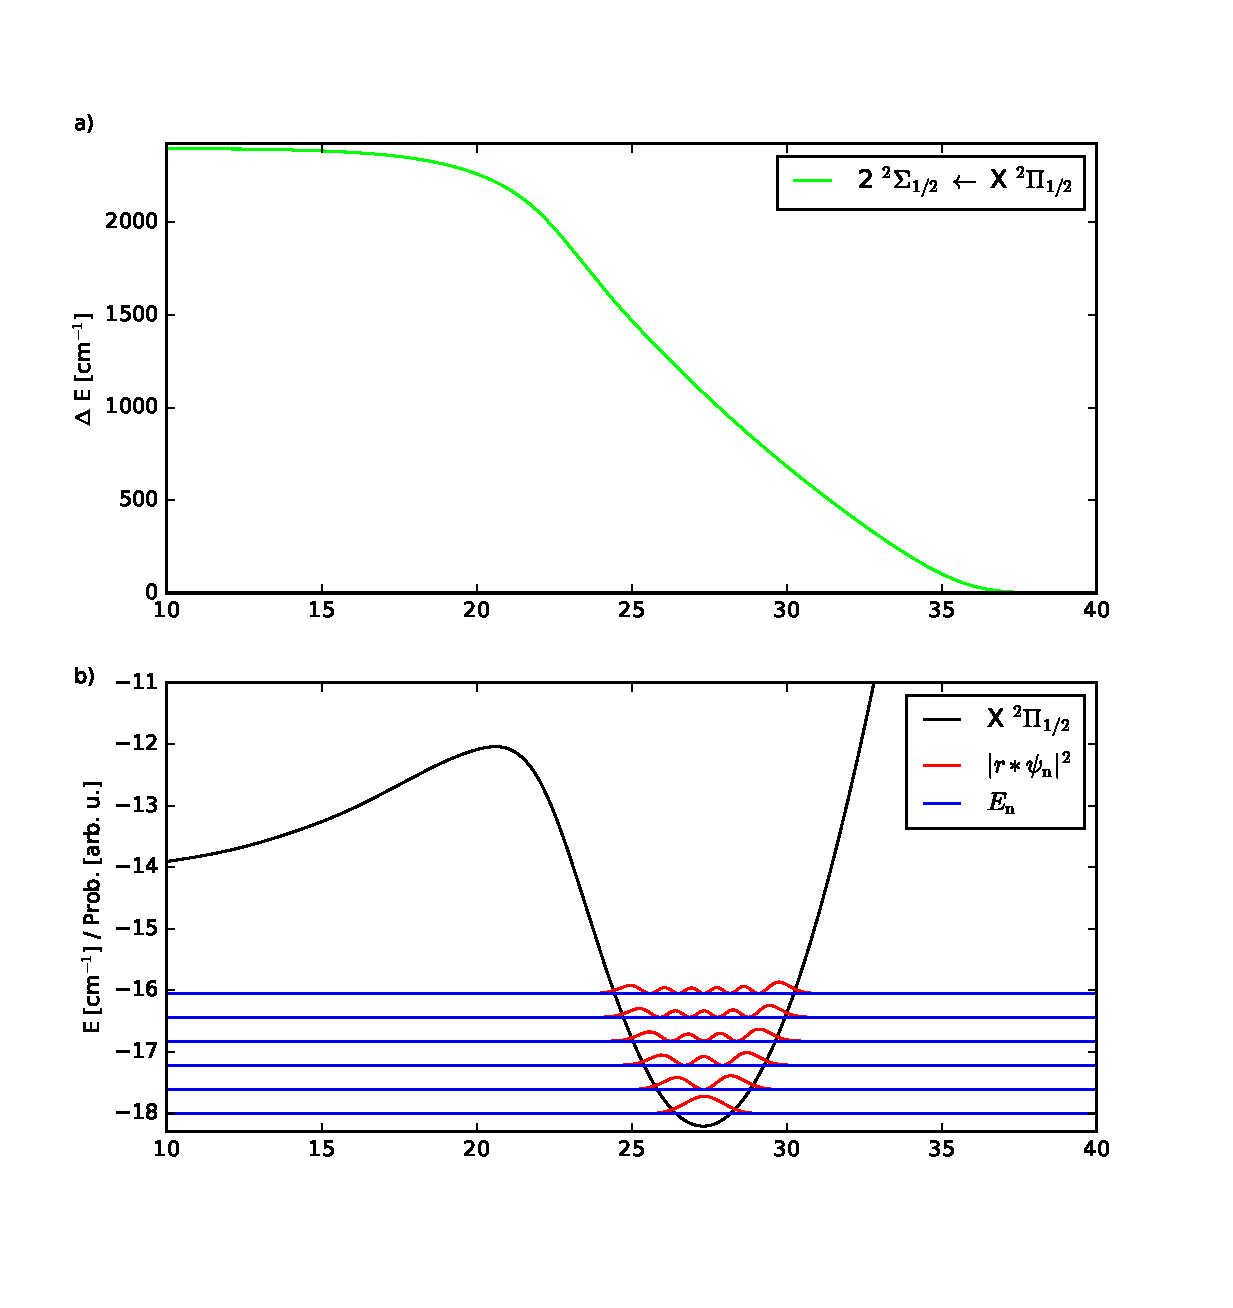
\includegraphics[width=0.45\textwidth]{6.eps}
                \caption{The upper plot (a) depicts the correction energy $\Delta{}E$ obtained in the frozen-droplet approximation for the  6s$\leftarrow{}$5p transition of In. It can be interpreted as the extra energy needed to form the electronically excited state in the He environment of the relaxed ground state of the atom. The lower plot (b) shows the near-surface minimum of the potential energy surface for ground state In in He$_{2000}$, together with the first few vibrational states and their corresponding probability densities. The latter are used as weights in the calculation of the blueshifted transition line. \label{pic:extra}}
  	\end{center}
\end{figure}

In the third and final step we use this curve of extra energy to estimate the position and the width of the perturbed electronic excitation for a direct comparison to the experiment. In order to do this, we solve the nuclear Schr\"odinger equation for the motion of the In atom in its electronic ground state potential to obtain the first few vibrational levels. The corresponding differential equation is solved numerically via finite differences and a discretization of the radial distance $z$ in the diatomic picture. Assuming a Boltzmann distribution at 0.37~K, the temperature of the He droplet, for the occupation of the vibrational levels, we then calculate an averaged probability $\rho{}_{\rm av}(z)$ from the corresponding nuclear wavefunctions and use this result to obtain an estimate for the perturbed  6s$\leftarrow{}$5p transition via an integration over vertical transitions at different $z$ positions weighted with $\rho{}_{\rm av}(z)$,
\begin{equation}
\bar{I}(\nu) = I(\nu) +  \int_{0}^{\infty} \mathrm{d}z\,\rho{}_{\rm av}(z) \Delta{}E(z),
\end{equation}
with  $I(\nu)$ denoting the intensity of the unperturbed electronic excitation as a  function of the frequency $\nu$ and $\bar{I}(\nu)$ as the final, perturbed spectrum. The result of this approximation is shown in Figure~\ref{pic:final}.

\begin{figure}[htbp!]
  	\begin{center}
 		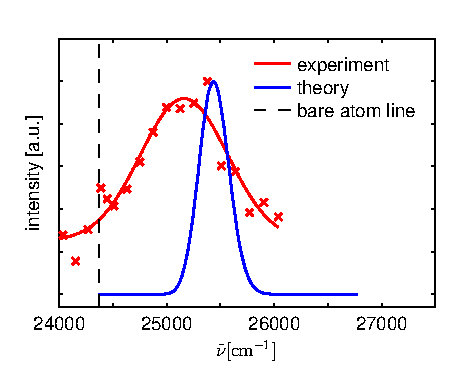
\includegraphics[width=0.45\textwidth]{7.eps}
                \caption{Comparison of the experimentally observed and the simulated 6s$\leftarrow{}$5p transition of In in He$_{2000}$. The blueshift is nicely reproduced by the frozen-droplet assumption, deviating from the experimental line position by less than 300~cm$^{-1}$. \hl{Lieber Johann, hier bitte aktualisieren, sobald die Experimentatoren uns die Daten fuer den Peak schicken.} \label{pic:final}}
  	\end{center}
\end{figure}

\section{Conclusion}
In this article we studied the blueshift of the 6s$\leftarrow{}$5p transition of atomic indium in helium nanodroplets. The experimental finding could be explained by a combination of quantum chemistry calculations and helium density functional theory. It is a consequence of the extra cost for the electronic excitation of the In atom, which is almost completely immersed in the helium in its electronic ground state, forming a pronounced dimple on the droplet surface. Upon excitation, the interaction with the surrounding helium becomes fully repulsive and the In atom is removed from the droplet. Within the frozen droplet approximation, and assuming that the total interaction is well approximated by the summation over pair interactions, the extra energy needed for the excitation can be estimated from the He-In potential curve for the  $^2\Sigma_{1/2}$ state (corresponding to the $^2S_{1/2}$ excited state of the In atom) via an integration over the unrelaxed or `frozen' helium density of the system obtained for the electronic ground state of indium. Taking into consideration also the motion of the In atom in the electronic groundstate, we can reproduce the shift and the broadening of the atomic 6s$\leftarrow{}$5p transition due to the helium environment.

%\renewcommand\refname{Notes and references}

%%%REFERENCES%%%
\bibliography{indi} %You need to replace "rsc" on this line with the name of your .bib file
\bibliographystyle{rsc} %the RSC's .bst file

\end{document}
